\section{Kapitel 2}
%TODO by Selina/Christian

\subsection{Begriffe}
Phasenraum/Vektorfeld usw...
\subsection{Bilanzieren}
\subsection{Matrixdarstellung}
$x' = Ax + b$\\
Kritische Punkte: $x' = Ax + b = 0$ Gleichgewicht: $b = -Ax$ oder $x = -A^{-1}*b$\\
Lösungen bei b=0 (homogenen Gleichung): Für jeden Eigenwert und Eigenvektor eine Lösung: \\
$x_1(t) = e^{\lambda_1t}v_1,x_2(t) = e^{\lambda_2t}v_2...x_n(t) = e^{\lambda_nt}v_n$\\

\subsection{Variation der Konstanten}
Gegeben ist ein lineares, inhomogenes System 1. Ordnung: \\
\begin{equation*}
\frac{d}{dt}x(t) = Ax(t) + b(t) 
\end{equation*}
Als erstes werden die Lösungen der homogenen Gleichung gelöst, wir erhalten für jeden Eigenwert und Eigenvektor eine Lösung: \\
$x_1(t) = e^{\lambda_1t}v_1,x_2(t) = e^{\lambda_2t}v_2...x_n(t) = e^{\lambda_nt}v_n$\\
Diese Lösungen ergeben unsere Fundamentalmatrix:\\
\begin{equation*}
X(t) = 
	\begin{bmatrix} 
	        x_1(t) && x_2(t) && ... && x_n(t)\\    
	\end{bmatrix}
\end{equation*}

Mit Hilfe der Fundamentalmatrix können wir nun die partikuläre Lösung des Systems bestimmen:\\
\begin{equation*}
y_P(t) = X(t) \int{X(t)^{-1}b(t)dt}
\end{equation*}
Die gesamte Lösung ist nun die Summe der homogenen und der partikulären Lösung.

\newpage
\subsection{Superpositionsprinzip}
Gegeben ist folgendes lineares homogenes Gleichungssystem:
\begin{equation*}
\frac{d}{dt}x(t) = A(t)x(t)
\end{equation*}
Das Superpositionsprinzip sagt, dass die Linearkombination der beiden Lösungen $x_1(t)$ und $x_2(t)$ auch wieder eine Lösung des Differentialgleichungssystems ist. 
\begin{equation*}
	x(t) = c_1 x_1(t) + c_2 x_2(t)
\end{equation*}
Wobei $c_1$ und $c_2$ beliebige Skalare sind. 
Das Prinzip kann auch für Systeme höherer Ordnung verwendet werden. \\

Hier ein \textbf{Beispiel} für eine Differentialgleichung zweiter Ordnung: \\
Gegeben: $t^2y''(t)-4ty'(t)+6y(t)=0$, $t>0$, $y_1(t)=t^2$\\
Gesucht: Eine zweite Lösung $y_2(t)$, so dass ${y_1(t),y_2(t)}$ ein Fundamentalsystem ergeben. \\
Vorgehensweise: \\
\textbf{Schritt 1:}\\
Prüfen, ob $y_1(t)$ wirklich Lösung des Systems ist. \\
\textbf{Schritt 2:}\\
Für die zu bestimmende Lösung $y_2(t)$ kommt folgender Ansatz zum Zug: $y_2(t) = v(t)y_1(t)$.\\
\textbf{Schritt 3:}\\
Ansatz $v(t)y_1(t)$ in Differentialgleichung einsetzen. Die Gleichung so weit es geht umformen und danach nach $v(t)$ auflösen. Wenn $v(t)$ bekannt ist, kann $y_2(t)$ berechnet werden. \\
\textbf{Schritt 4:}\\
Auf Grund der beiden Lösungen, kann die Fundamentalmatrix $Y(t) =
\begin{vmatrix} 
	        y_{1}(t) & y_{2}(t)\\ 
	        y'_{1}(t) & y'_{2}(t)\\   
\end{vmatrix} $ berechnet werden und mit Hilfe der Wronskideterminante geprüft werden, ob die Lösungen linear unabhängig sind ($det(W) \neq 0$). 

\subsection{Lineare Unabhängigkeit}
Die lineare Unabhängigkeit der beiden Lösungen $x_1(t)$ und $x_2(t)$ kann mit Hilfe der \textbf{Wronskideterminante} geprüft werden. 
\begin{equation*}
	W(t) = det[X(t)] =    
	\begin{vmatrix} 
	        x_{11}(t) & x_{12}(t)\\ 
	        x_{21}(t) & x_{22}(t)\\   
	\end{vmatrix}
\end{equation*}
Sind $x_1(t)$ und $x_2(t)$ \textbf{linear unabhängig}, dann gilt $W(t) \neq 0$ für alle $t \in I$. \\
Sind $x_1(t)$ und $x_2(t)$ \textbf{linear abhängig}, dann gilt $W(t) = 0$ für alle $t \in I$. \\
Jede Lösung $\Phi(t)$ kann als Linearkombination eines Fundamentalsystems zweier Lösungen $x_1(t)$ und $x_2(t)$ dargestellt werden. Diese Linearkombination wird als die allgemeine Lösung eines linearen homogenen Systems bezeichnet. \\
\textbf{Theorem von Abel}\\
\begin{equation*}
W(t) = c\cdot e^{\int{\operatorname{trace}(A(t))dt}}
\end{equation*}
Spur einer Matrix = Summe der Hauptdiagonalelemente
\subsection{Fluss eines Vektorfeldes}
Die Matrix A ordnet jedem Vektor x einen Vektor A(x) des Vektorfeldes zu. Der Fluss $\Phi(t)$ transformiert jeden Anfangszustand $x_0$ längs der druch $x_0$ verlaufenden Trajektorie in den Zustand x(t) zur Zeit t. \\
Es gelten folgende Zusammenhänge:\\
\begin{equation*}
\Phi(t) = X(t)X(t_0)^{-1}
\end{equation*}

\begin{equation*}
\Phi(t)X(t_0) = X(t)
\end{equation*}

\begin{equation*}
\Phi'(t) = A(t)\Phi(t)
\end{equation*}

\begin{equation*}
\Phi(t_0) = E
\end{equation*}

\begin{equation*}
\Phi(t) = e^{A(t)t} =\sum_{k=0}^{\infty}\frac{(A(t)\cdot t)^k}{k!}
\end{equation*}

Beispiele:\\
Gegeben: $A = 	\begin{vmatrix} 
	        		\lambda & 0\\ 
	        		0 & \lambda\\   
				\end{vmatrix} 
				\rightarrow$ 
$e^{tA} = \begin{vmatrix} 
	        		e^{t\lambda} & 0\\ 
	        		0 & e^{t\lambda}\\   
				\end{vmatrix}$\\
Gegeben: $A = 	\begin{vmatrix} 
	        		\lambda & 1\\ 
	        		0 & \lambda\\   
				\end{vmatrix} 
				\rightarrow$ 
$e^{tA} = \begin{vmatrix} 
	        		e^{t\lambda} & te^{t\lambda}\\ 
	        		0 & e^{t\lambda}\\   
				\end{vmatrix}$\\
				
Gegeben: $A = 	\begin{vmatrix} 
	        		2 & 3\\ 
	        		3 & 2\\   
				\end{vmatrix} \rightarrow
				\lambda_1=5 \; \lambda_2=-1 \rightarrow ev_1=\begin{vmatrix}
					1\\ 
					1\\   
				\end{vmatrix} \;
				ev_2=\begin{vmatrix}
					1\\ 
					-1\\   
				\end{vmatrix} \rightarrow
				T=\begin{vmatrix} 
	        		1 & 1\\ 
	        		1 & -1\\   
				\end{vmatrix} \rightarrow 
				B=T^{-1} \cdot A \cdot T=\begin{vmatrix} 
	        		5 & 0\\ 
	        		0 & -1\\   
				\end{vmatrix} \rightarrow$\\
				\hspace*{4cm}$e^{tA}=T \cdot e^{tB} \cdot T^{-1}=
				T \cdot \begin{vmatrix} 
					e^{5 t} & 0\\ 
					0 & e^{-t}\\   
				\end{vmatrix} \cdot T^{-1} =
				\dfrac{1}{2}\begin{vmatrix} 
					e^{5 t} + e^{-t}& e^{5 t} - e^{-t}\\ 
					e^{5 t} - e^{-t} & e^{5 t} + e^{-t}\\   
				\end{vmatrix}$


%Das Vektorfeld lässt sich auch aus dem Fluss zurück gwinnen, indem die Trajektorie $\phi(t) = \Phi(t)x$ nach er Zeit an der Stelle $t=0$ abgeleitet
%Gegeben ist ein autonomes lineares homogenes System mit einer nxn Matrix A:
%\begin{equation*}
%\frac{d}{dt}x(t) = A(t)x(t)
%\end{equation*}
%Die Matrix $A(t)$ besitzt verschiedene reelle Eigenwerte. Aus den Eigenwerten $\lambda_1$ und $\lambda_2$ und ihren zugehörigen Eigenvektoren $\nu_1$ und $\nu_2$ erhalten wir ein System von Fundamentallösungen: 
%\begin{equation*}
%x_1(t) = e^{\lambda_1t}\nu_1\\
%\end{equation*}
%\begin{equation*}
%x_2(t) = e^{\lambda_2t}\nu_2
%\end{equation*}
%Die Fundamentallösungen $x_1(t)$ und $x_2(t)$ bilden die Spalten der Fundamentalmatrix $X(t)$:
%\begin{equation*}
%	X(t) =     
%	\begin{vmatrix} 
%	        x_{11}(t) & x_{12}(t)\\ 
%	        x_{21}(t) & x_{22}(t)\\   
%	\end{vmatrix}
%\end{equation*}
%Diese Fundamentalmatrix genügt folgender Differentialgleichung: 
%\begin{equation*}
%\frac{d}{dt}X(t) = A(t)X(t)
%\end{equation*}
%Fluss? Versteh ich nicht so ganz. 
%
%Die Lösung x(t) des Anfangswertproblems $x(t_0) x_0$ kann mit Hilfe einer Fundamentalmatrix X(t) dargestellt werden. Die allgemeine Lösung der Diffgleichung $\frac{d}{dt}x(t) = A(t)x(t)$ kann als Superposition von Fundamentallösungen  geschrieben werden.\\
%\begin{equation*}
%x(t) = c_1 x_1(t) + ... + c_n x_n(t)
%\end{equation*}
%\begin{equation*}
%x(t) = X(t)c
%\end{equation*}
%Mit $x_0 = X(t_0)$ und $det(X(t_0)) \neq 0$
%\begin{equation*}
%c = X(t_0)^{-1}x_0
%\end{equation*}
%In obige Gleichung eingesetzt, ergibt: 
%\begin{equation*}
%x(t) = X(t)X(t_0)^{-1}x_0
%\end{equation*}
%Wählt man nun die Fundamentallösungen $x_1(t) ... x_n(t)$ zu den Anfangsbedingungen $x_1(t_0)=e_1, ..., x_n(t_0)=e_n$, wobei $e_1...e_n$ die kanonischen Basisvektoren des Vektorraumes $R^n$ sind, erhalten wir die zugehörige Fundamentalmatri:
%\begin{equation*}
%\Phi(t_0) = E
%\end{equation*}
%Es folt aus dem Eindeutigkeitssatz, dass die Lösung x(t) des Anfangswertproblems $x(t_0) = x_0$ mit Hilfe dieser speziellen Fundamentalmatrix $\Phi(t)$, folgende Darstellung besitzt: 
%\begin{equation*}
%x(t) = \Phi(t)x_0
%\end{equation*}
%mit $\Phi(t) = X(t)X(t_0)^{-1}$. In Worten: Die Matrix A ordnet jedem Vektor x einen Vektor A(x) des Vektorfeldes zu. Der Fluss $\Phi(t)$ transformiert jeden Anfangszustand $x_0$ längs der druch $x_0$ verlaufenden Trajektorie in den Zustand x(t) zur Zeit t. 
%Das Vektorfeld lässt sich auch aus dem Fluss zurück gwinnen, indem die Trajektorie $\phi(t) = \Phi(t)x$ nach er Zeit an der Stelle $t=0$ abgeleitet wird. 
%\begin{equation*}
%\frac{d}{dt}\Phi(t)x = A(x)
%\end{equation*}

\subsection{Matrixexponential}
Gegeben ist die Differentialgleichung:
\begin{equation*}
\frac{d}{dt}x(t) = A(t)x(t)
\end{equation*}
mit Anfangsbedingung $x(0) = x_0$ und der konstanten $n \times n$ Matrix A. Mit Hilfe des Flusses $\Phi(t)$ kann die Lösung dieses Problems dargestellt werden als: 
\begin{equation*}
x(t) = \Phi(t)x_0
\end{equation*}
Bei einer skalaren Differentialgleichung $\frac{d}{dt}x(t) = ax(t)$ ist die Lösung bei gegebener Anfangsbedingung: $x(t) = e^{at}x_0$. Wenn wir diese Lösung nun mit $\Phi(t)$ vergleichen, stellt sich heraus, dass der Fluss eines $n \times n$ Systems ebenfalls eine Exponentialdarstellung besitzt. 
Ist $A$ eine konstante $n \times n$ Matrix, dann besittz der Fluss $\Phi(t)$, der vom Vektorfeld erzeugt wird, folgende Darstellung als Matrixexponential: 
\begin{equation*}
\Phi(t) = e^{At} = X(t)X(0)^{-1}
\end{equation*}
Der Fluss wie auch das Matrixexponential können also mit Hilfe der Fundamentalmatrix X(t) und der entsprechenden Anfangsbedingung berechnet werden.
Damit hat die Lösung x(t) des Anfangswertproblems $x(0) = x_0$ folgende Form: 
\begin{equation*}
x(t) = e^{At}x_0
\end{equation*}


\subsection{Degenerierte Matrizen}
Ist $A$ degeneriert, bedeutet dies, dass sie mindestens einen Eigenwert $\lambda$ mit einer geometrischen Vielfachheit (Anzahl Eigenvektoren) besitzt, die kleiner als seine algebraische Vielfachheit (Anzahl gleiche Eigenwerte $m$) ist. 
Das bedeutet, dass die linear unabhängigen Eigenvektoren der Matrix $A$ den Raum $\mathbb{R}^n$ nicht ausschöpft.\\
Ist $\lambda$ ein Eigenwert von $A$ mit der algebraischen Vielfachheit $m$, dann besitzt die Gleichung: 
\begin{equation*}
(A-\lambda E)^m b_k = 0
\end{equation*}
eine Anzahl $m$ linear unabhängige Lösungen $b_1$ bis $b_m$ und für $k = 1,\ldots,m$ sind die vektorwertigen Funktionen
\begin{equation*}
x_k(t) = e^{\lambda t}\left[{b_k + \frac{t}{1!}(A-\lambda E)b_k + ... + \frac{t^{m-1}}{(m-1)!}(A-\lambda E)^{m-1}b_k}\right]
\end{equation*}
\begin{equation*}
 \Longrightarrow x_k(t) = e^{\lambda t}(b_k + t (A-\lambda E) b_k))
\end{equation*}
linear unabhängige Lösungen der Differentialgleichung. 
\subsection{Beispiel}
Folgende Matrix A ist gegeben: 
\begin{equation*}
	A =     
\begin{bmatrix} %phantom is for spacing
	2 & 0 & -1\\
	0 & 3 & 1\\
	0 & 0 & 2\\
\end{bmatrix}
\end{equation*}
\begin{equation*}
\det(A-\lambda E) = 0 \qquad \Longrightarrow \lambda_1 = 2 \text{(Doppelt)} \quad \lambda_2 = -1
\end{equation*}

\textbf{Schritt 1:} Eigenvektoren berechenen (Hier im Beispiel nur für $\lambda_1$)\\
\begin{equation*}
(A - \lambda_1 E)\nu = 0 \qquad \Longrightarrow \nu = 
\begin{bmatrix} %phantom is for spacing
	1 \\
	0 \\
	0 \\
\end{bmatrix}
\end{equation*}


\begin{equation*}
\Longrightarrow \text{Nur ein Eigenvektor aber zwei Eigenwerte $\lambda_1 = 2$} \quad \Longrightarrow m = 2
\end{equation*}
\textbf{Schritt 2:} Basisvektorern $b_k$ bestimmen \\
\begin{equation*}
(A-\lambda E)^2 b_k = 0 \qquad \Longrightarrow 0\cdot b_{k1} + 9\cdot b_{k2} - 3\cdot b_{k3} = 0
\end{equation*}
\begin{equation*}
b_1= 
\begin{bmatrix} %phantom is for spacing
	1 \\
	0 \\
	0 \\
\end{bmatrix}
\qquad b_2= 
\begin{bmatrix} %phantom is for spacing
	0 \\
	1 \\
	3 \\
\end{bmatrix}
\end{equation*}
\textbf{Schritt 3:} Lösung bestimmen\\
\begin{equation*}
x_1(t) = e^{2 \cdot t} (b_1 + t(A -  2 E)b_1) \qquad \Longrightarrow e^{2\cdot t}
\begin{bmatrix} %phantom is for spacing
	1 \\
	0 \\
	0 \\
\end{bmatrix}
\end{equation*}
\begin{equation*}
x_2(t) = e^{2 \cdot t} (b_2 + t(A -  2  E)b_2) \qquad \Longrightarrow e^{2\cdot t}
\begin{bmatrix} %phantom is for spacing
	-3t \\
	1 \\
	3 \\
\end{bmatrix}
\end{equation*}
\begin{equation*}
 \Longrightarrow X(t) = 
\begin{bmatrix} %phantom is for spacing
	 x_1(t) & x_2(t) \\
\end{bmatrix}
=
\begin{bmatrix} %phantom is for spacing
	1 \cdot e^{2 \cdot t} & -3t \cdot e^{2 \cdot t} \\
	0 & 1\cdot e^{2 \cdot t}  \\
	0 & 3 \cdot e^{2 \cdot t} \\
\end{bmatrix}
\end{equation*}


\subsection{Stabilit"at linearer Systeme}


\subsection{Entkoppeln}
\begin{minipage}[h]{0.35\textwidth}
Doppelter reeller Eigenwert:\\ Entkoppeln
\end{minipage}
\begin{minipage}[h]{0.5\textwidth}
	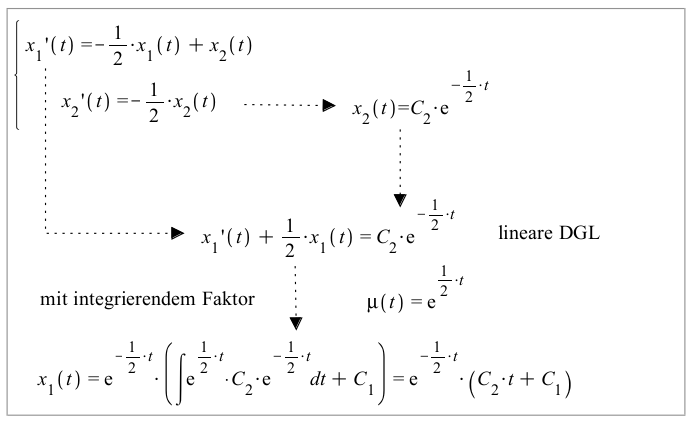
\includegraphics[width=1.0\textwidth]{images/Entkoppeln.png}
\end{minipage}

\subsection{ToDo}
- Superpositionsprinzip\\
- Fluss eines Vektorfeldes\\
- Degenerierte Matrizen\\
- Variation der Konstanten\\
